\chapter{CloudFront}\label{ch:cloudfront}

CloudFront will allow for the distribution of static and dynamic web images more efficiently.
An international network of data centres, referred to as edge locations, are used to deliver content for CloudFront.
An edge location which offers the lowest latency or delay in serving these files will be used.
This will involve the creation of a CloudFront Distribution.

Firstly, an origin is chosen which is the S3 bucket created in Section~\ref{ch:simple-storage-service}.
It is then given a name of \mintinline{zsh}|group4-digital-ink.s3.us-east-1.amazonaws.com|.
The "Yes use OAI" option is selected, in order to restrict bucket access to only CloudFront.
The "Bucket Policy" option is set to "Yes" to automatically update permissions on the bucket to allow read access for
the OAI.

\begin{figure}[!htbp]
    \centering
    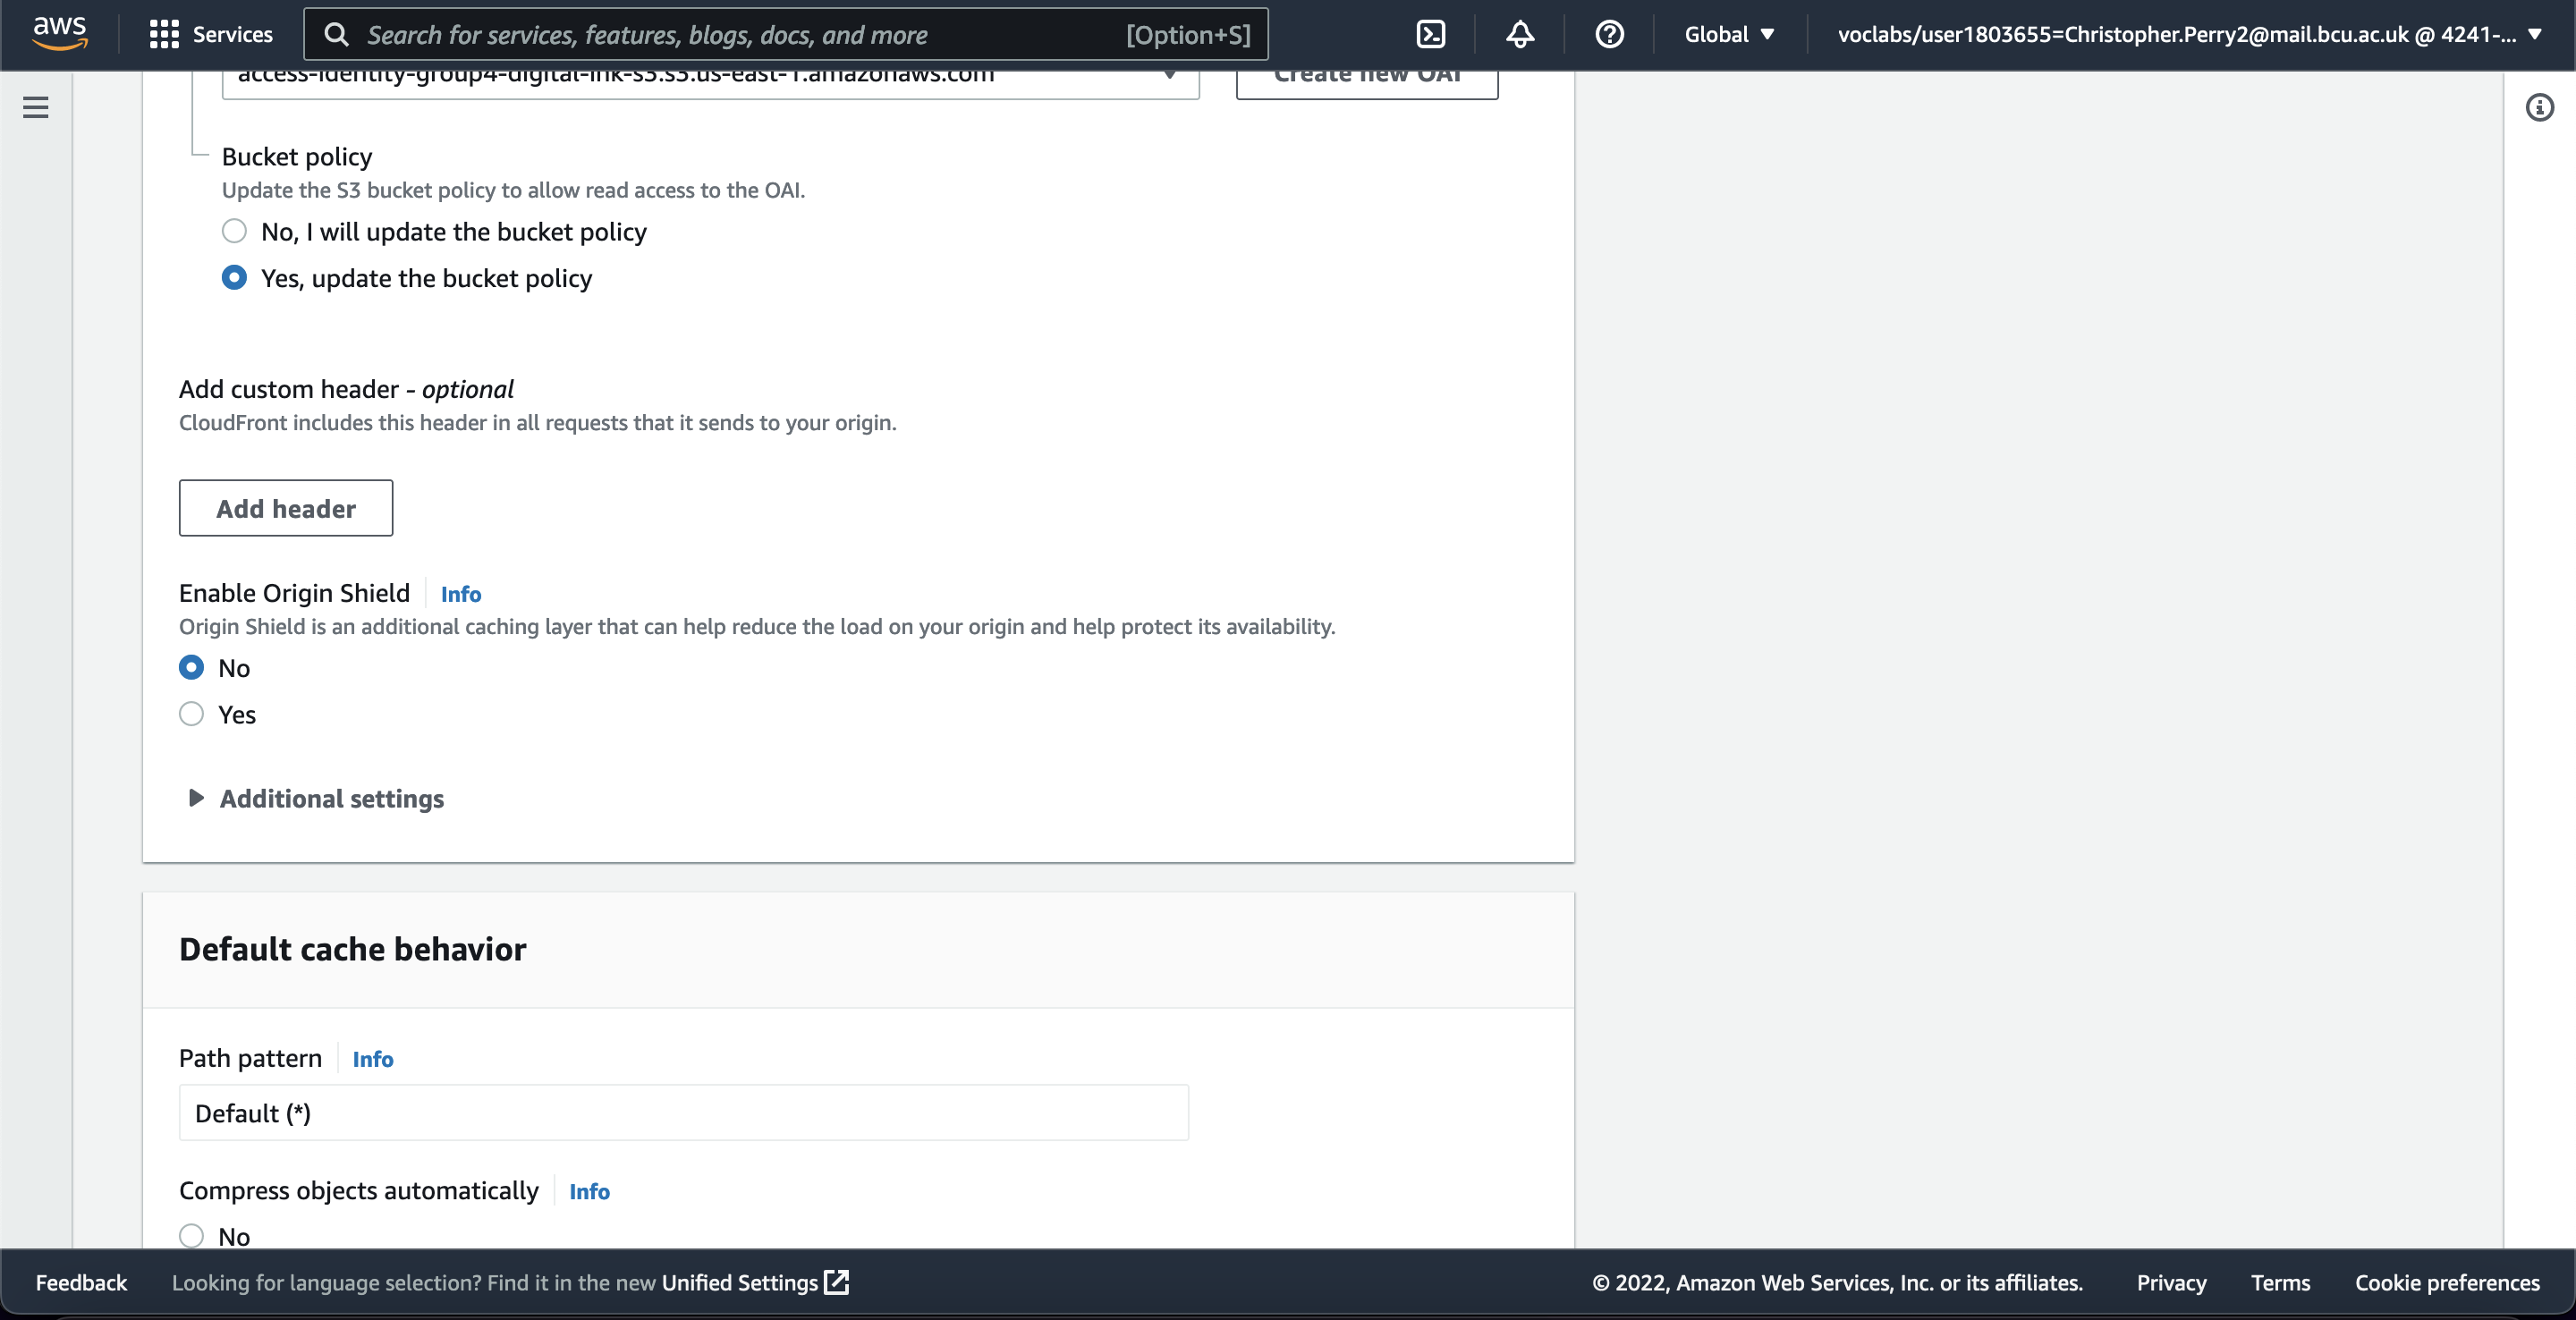
\includegraphics[width=\textwidth]{resources/cloudfront/cloudfront-bucket-policy}
    \caption{Applying CloudFront bucket policy.}
    \label{fig:cloudfront-bucket-policy}
\end{figure}

\begin{figure}[!htbp]
    \centering
    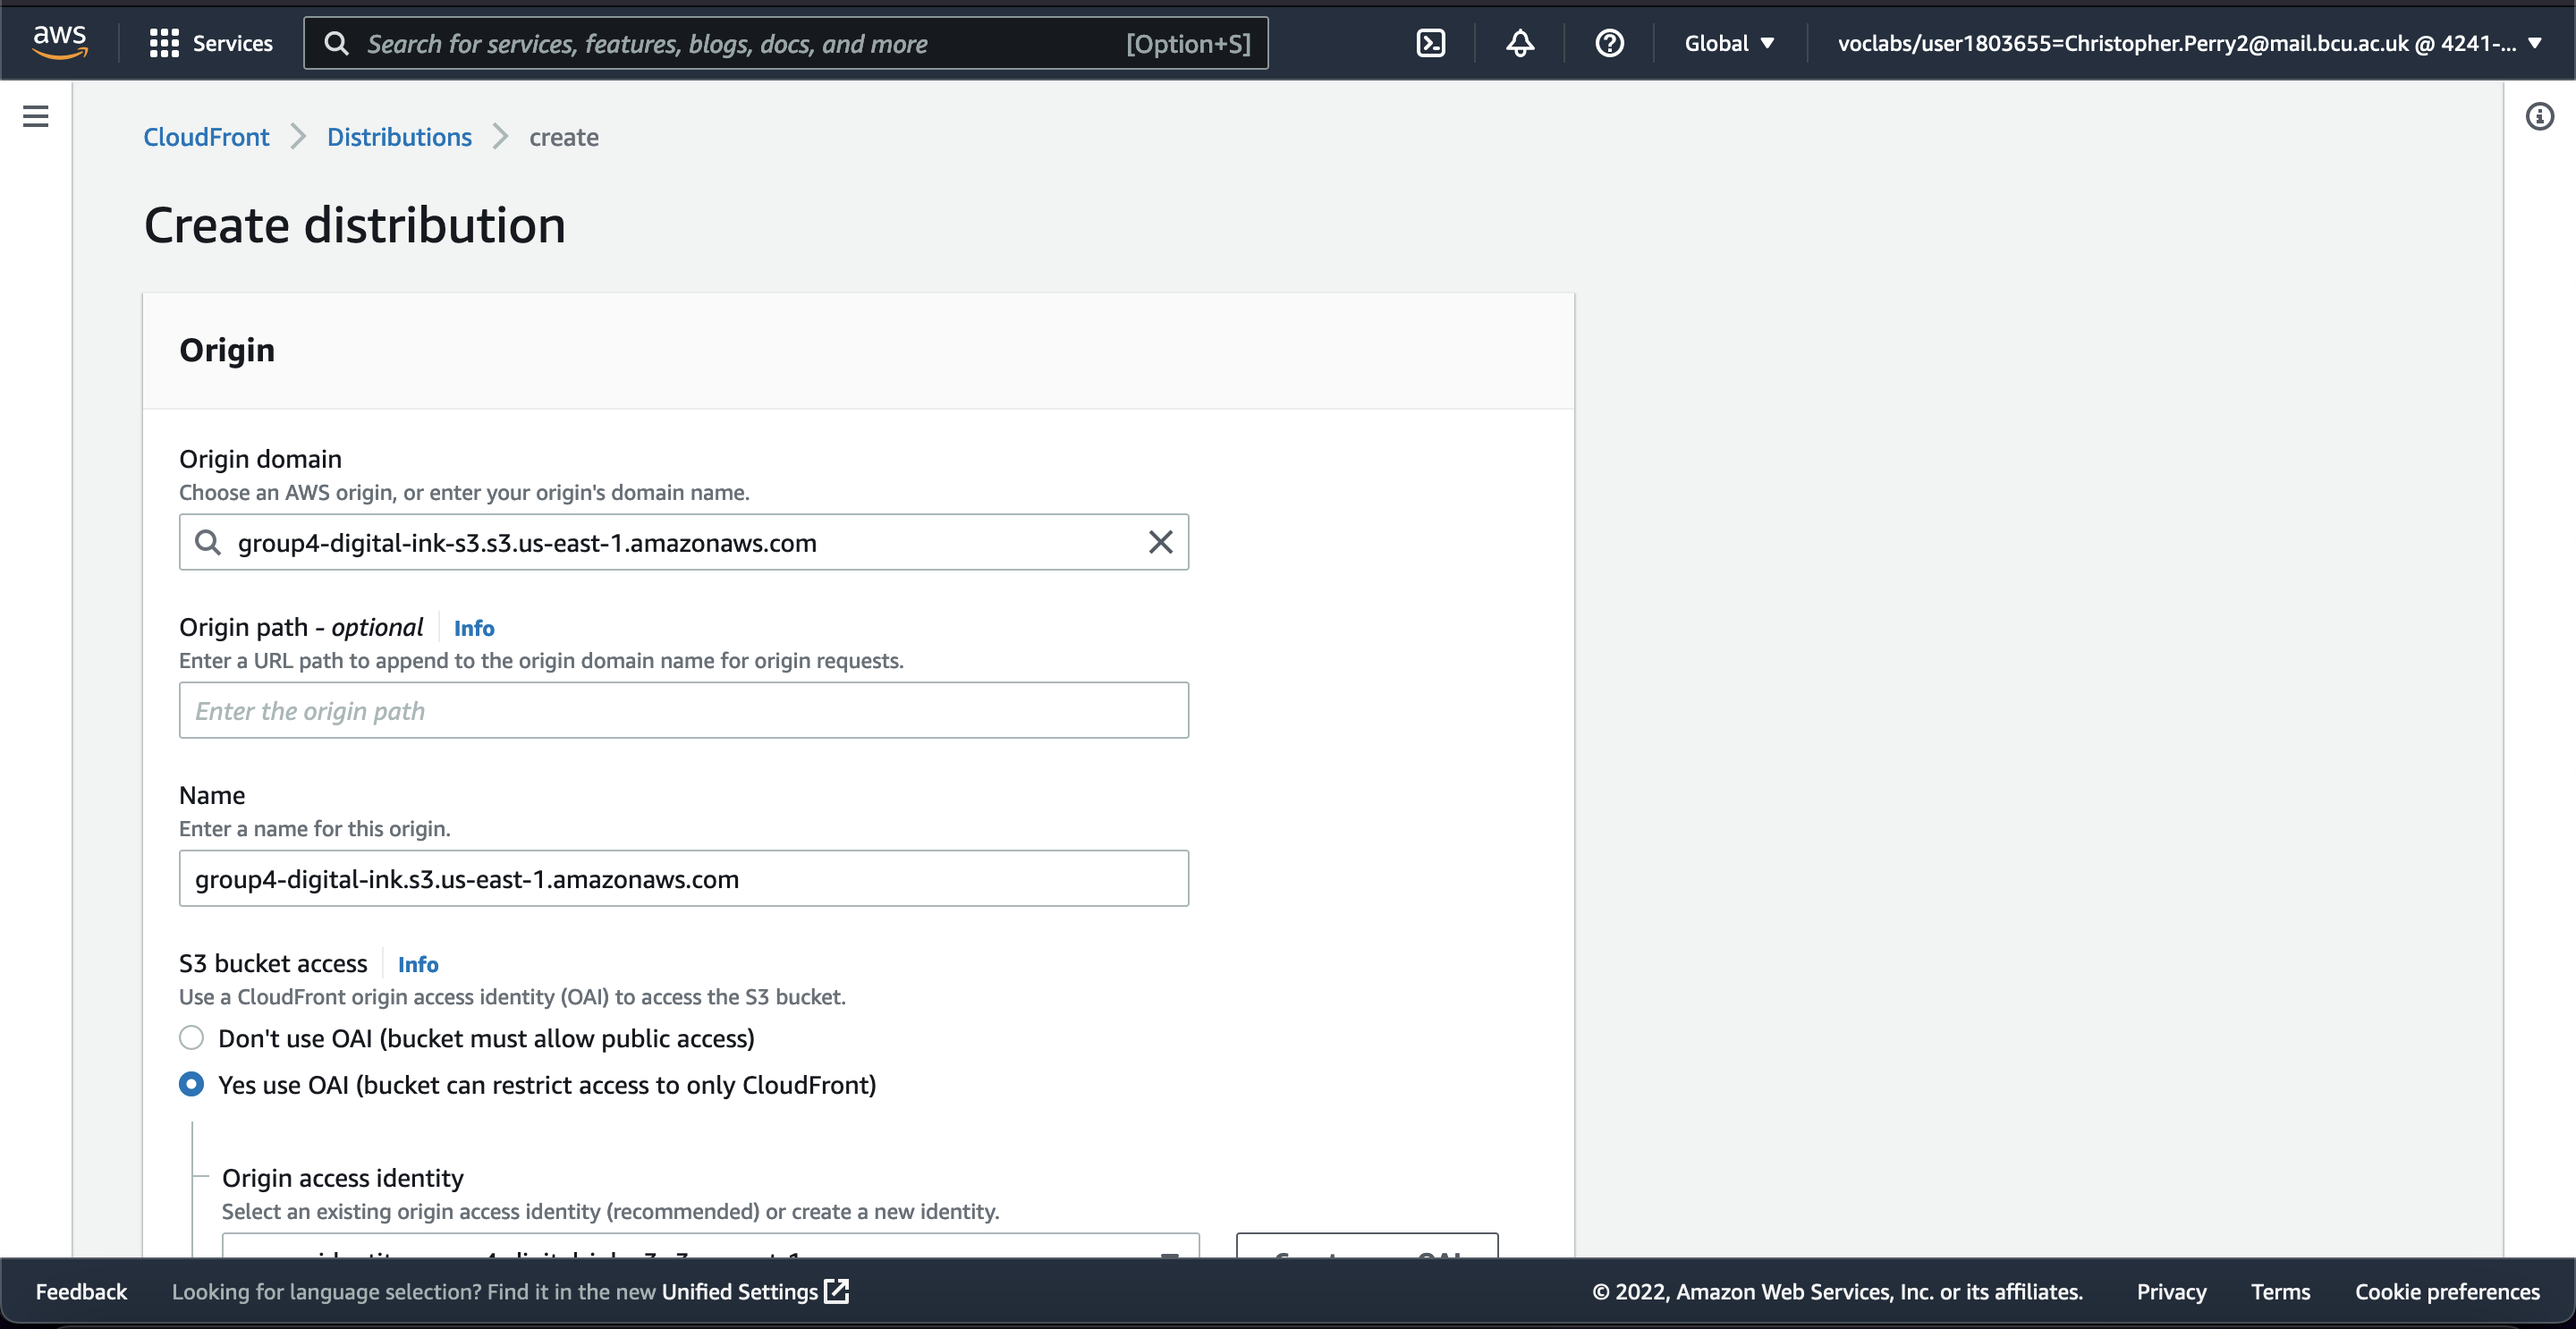
\includegraphics[width=\textwidth]{resources/cloudfront/cloudfront-origin}
    \caption{Applying CloudFront origins to S3 bucket.}
    \label{fig:cloudfront-origins}
\end{figure}

These options can be seen configured in Figures~\ref{fig:cloudfront-bucket-policy} and~\ref{fig:cloudfront-origins}.

Permissions are then applied to the CloudFront distribution itself.
Objects are set to be compressed automatically to save space, and for viewing images, permissions are set to be in
both HTTP and HTTPS, and to only allow \mintinline{zsh}|GET| and \mintinline{zsh}|HEAD|, so images can only be viewed.

\begin{figure}[!htbp]
    \centering
    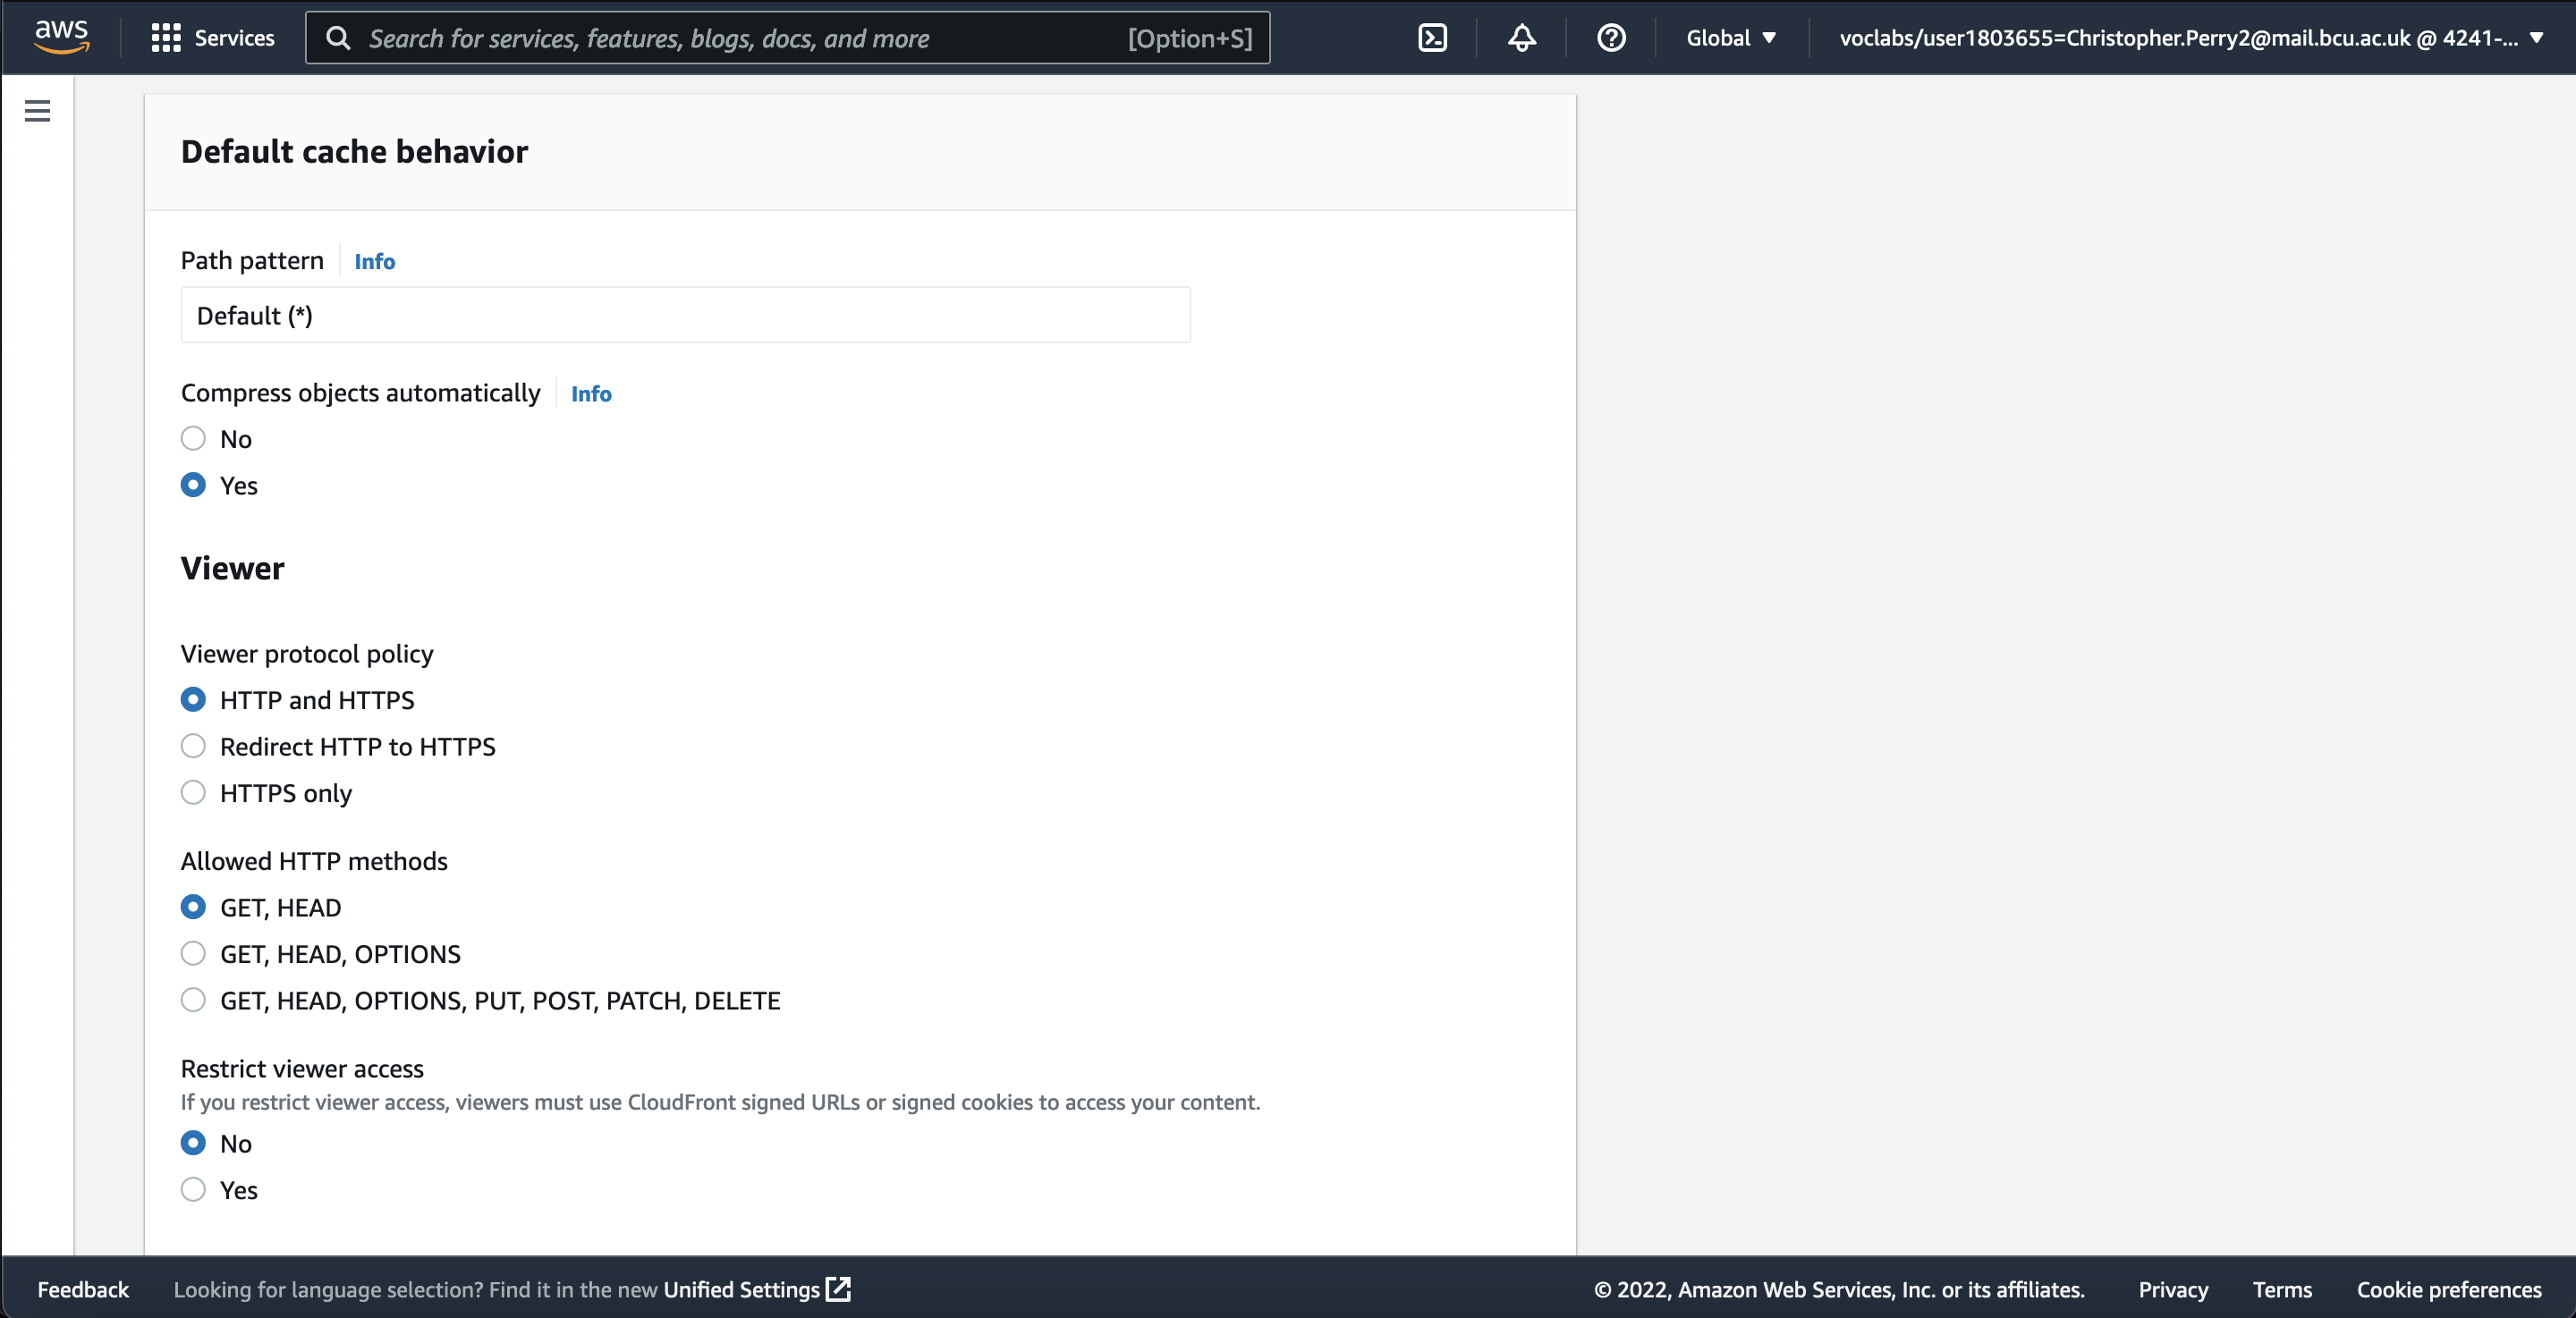
\includegraphics[width=\textwidth]{resources/cloudfront/cloudfront-cache-behaviour}
    \caption{Applying CloudFront Distribution Permissions.}
    \label{fig:cloudfront-cache-behaviour}
\end{figure}

A cache policy and origin request policy is subsequently applied to the aforementioned permissions.
The "CachingOptimized" policy is applied for compression.
Origin Request policy is set to "CORS-S3Origin" in order for CORS to be automatically set up for the S3 bucket,
Any GET requests are then compatible in the response headers through "SimpleCORS".

\begin{figure}[!htbp]
    \centering
    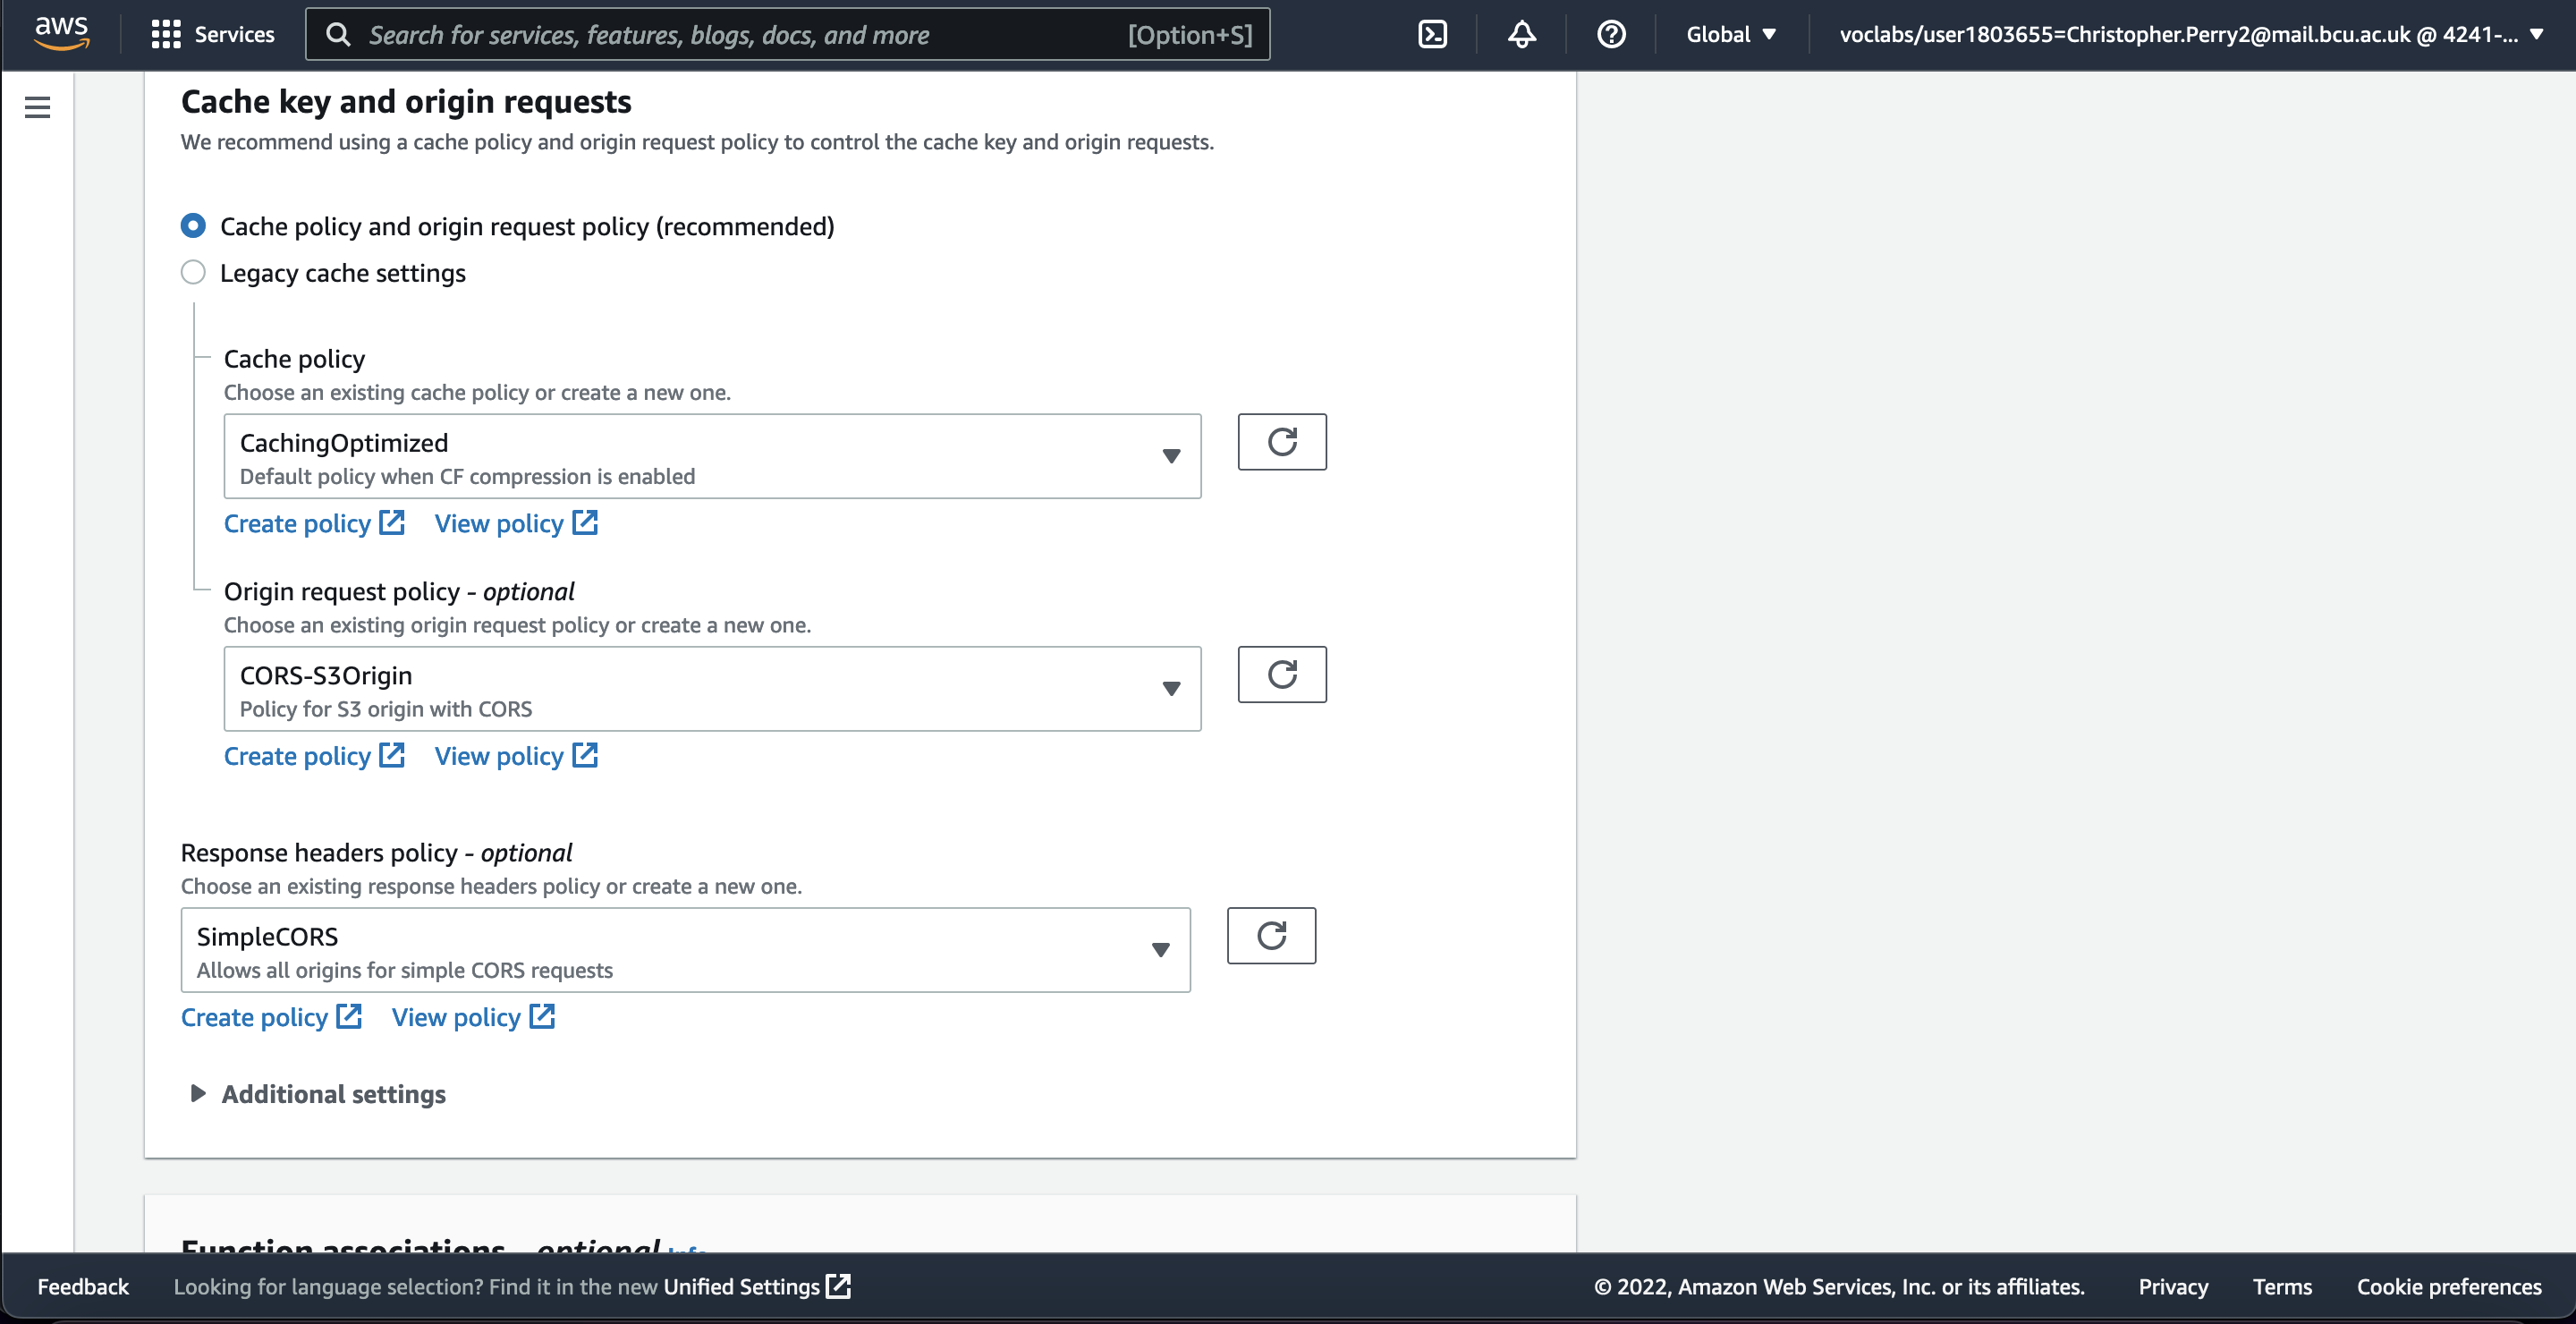
\includegraphics[width=\textwidth]{resources/cloudfront/cloudfront-cache-key}
    \caption{Applying CloudFront Cache Keys and Origin Requests.}
    \label{fig:cloudfront-cache-key}
\end{figure}

No function associations are set due to the lack of CloudFront functions and Lambdas.

\begin{figure}[!htbp]
    \centering
    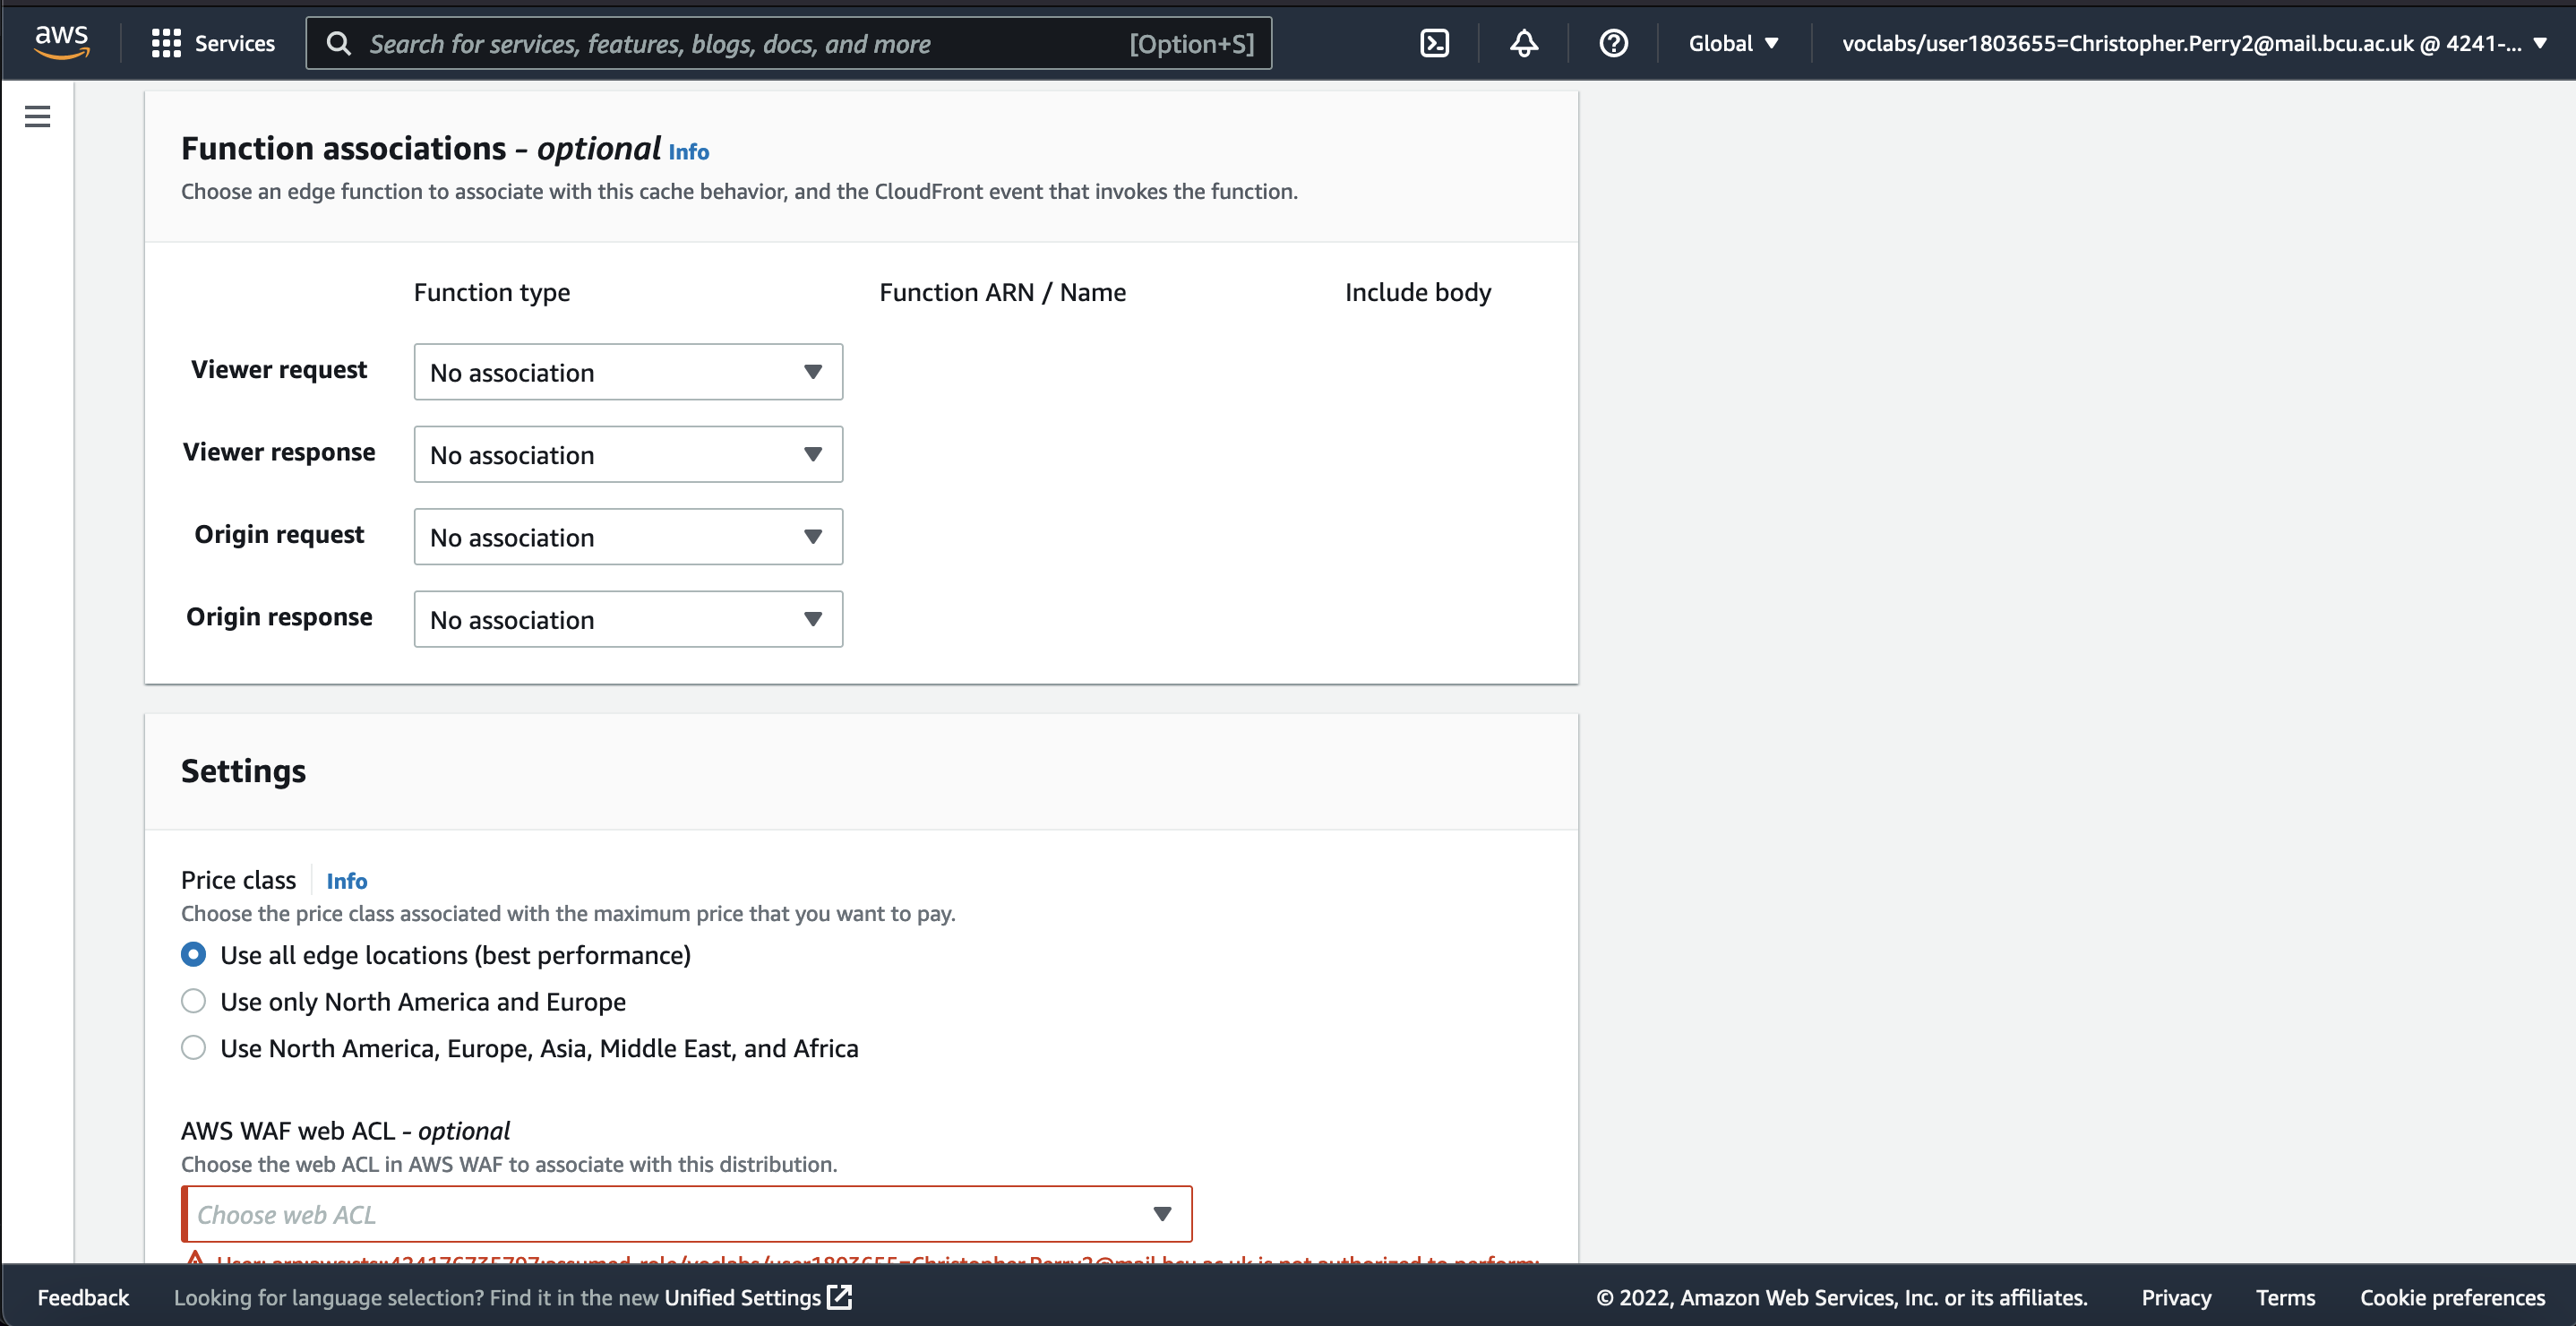
\includegraphics[width=\textwidth]{resources/cloudfront/cloudfront-function-association}
    \caption{Function Association.}
    \label{fig:cloudfront-function-association}
\end{figure}

The settings for the CloudFront Distribution can now be set.
In order to ensure high availability, the option "Use all edge locations" is selected, so that images can be distributed
to the user from the closest edge location in relation to their IP address.
No ACL can be added to the WAF due to permissions issues, and a SSL Certificate cannot be set as the web app is not being
served from the internet.
For logging purposes "Standard Logging" is set to "On", and logs are saved to the same S3 bucket.
Cookie logging is enabled, and IPv6 is set to "On", to allow for more IP addresses to access the CloudFront Distributed
content.

\begin{figure}[!htbp]
    \centering
    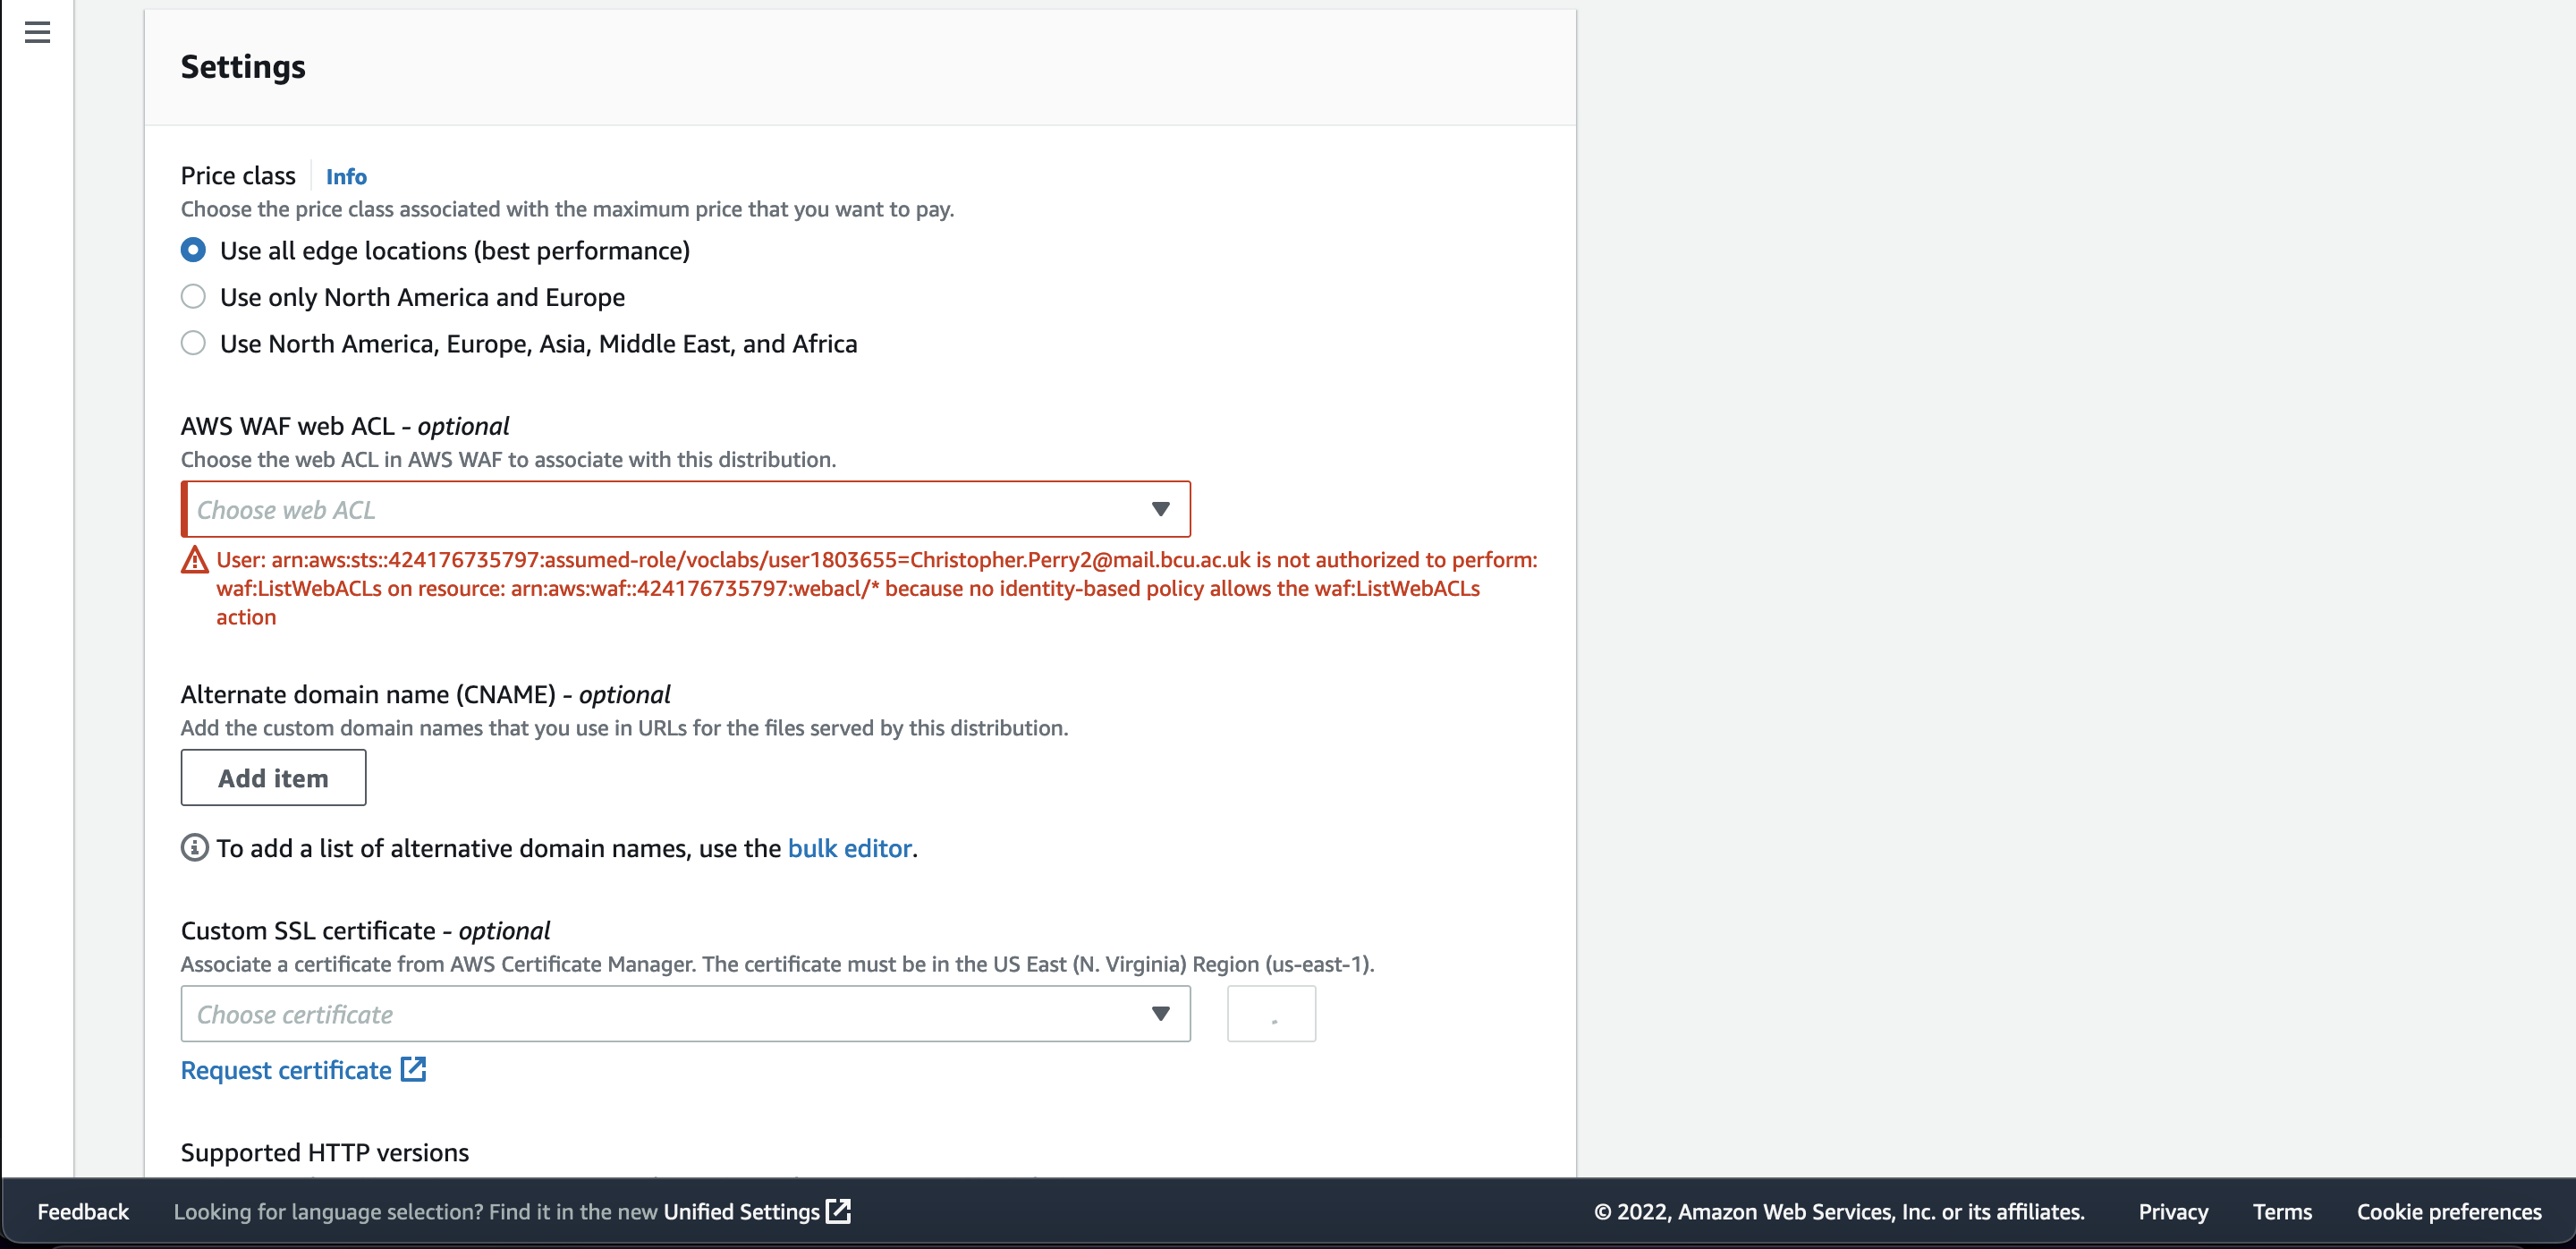
\includegraphics[width=\textwidth]{resources/cloudfront/cloudfront-settings-1}
    \caption{Applying CloudFront Settings.}
    \label{fig:cloudfront-settings-1}
\end{figure}

\begin{figure}[!htbp]
    \centering
    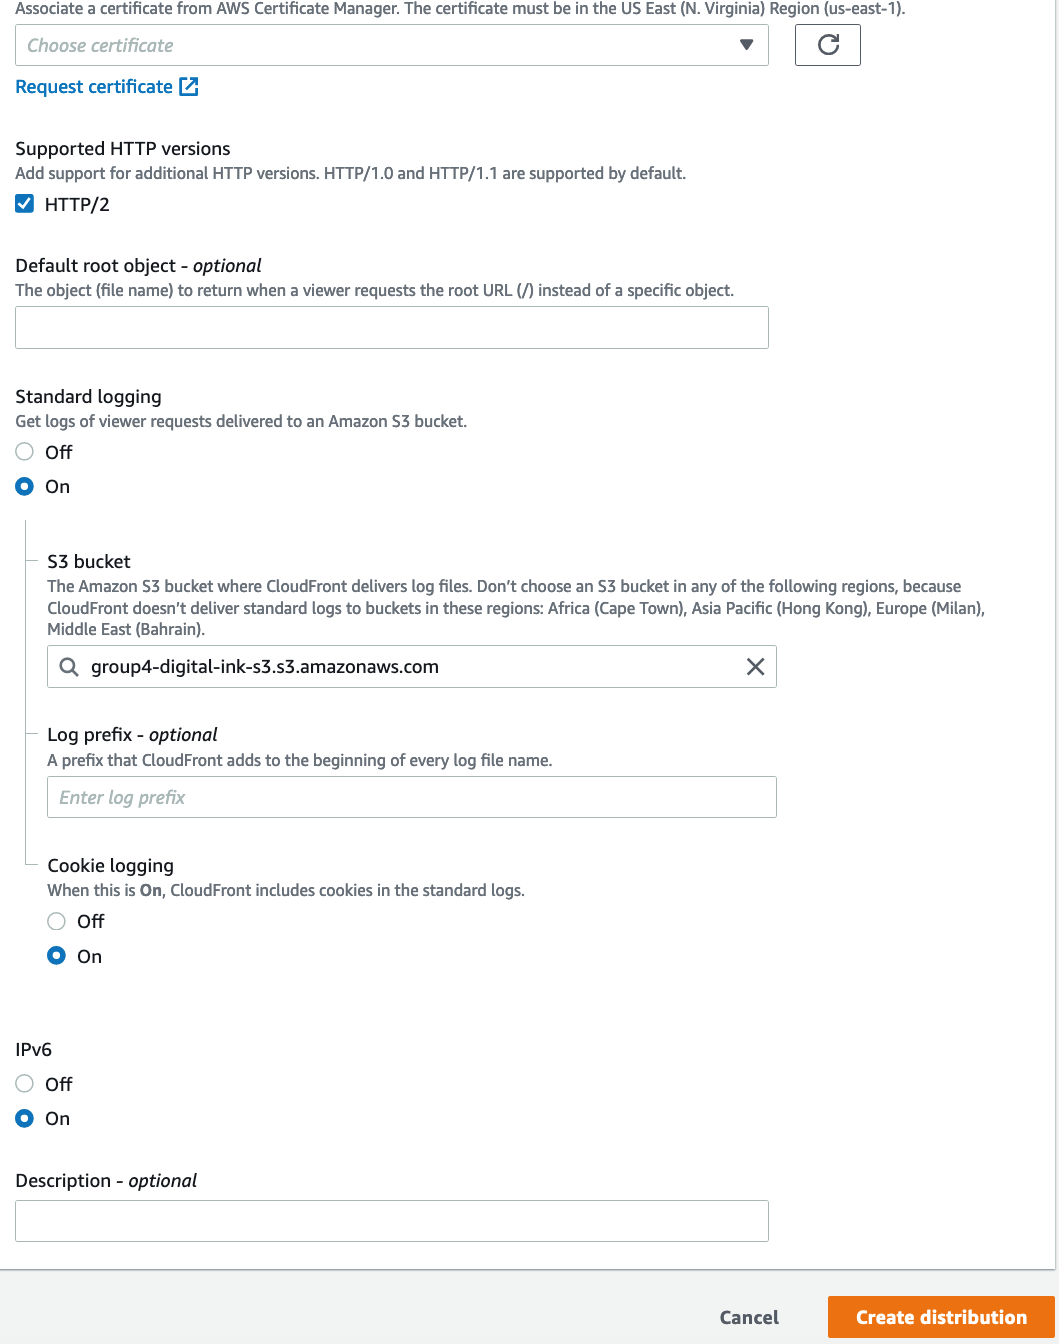
\includegraphics[width=\textwidth]{resources/cloudfront/cloudfront-settings-2}
    \caption{Applying CloudFront Settings.}
    \label{fig:cloudfront-setting-2}
\end{figure}

A CloudFront Distribution has now been created, and can be found in Figure~\ref{fig:cloudfront-created}.

\begin{figure}[!htbp]
    \centering
    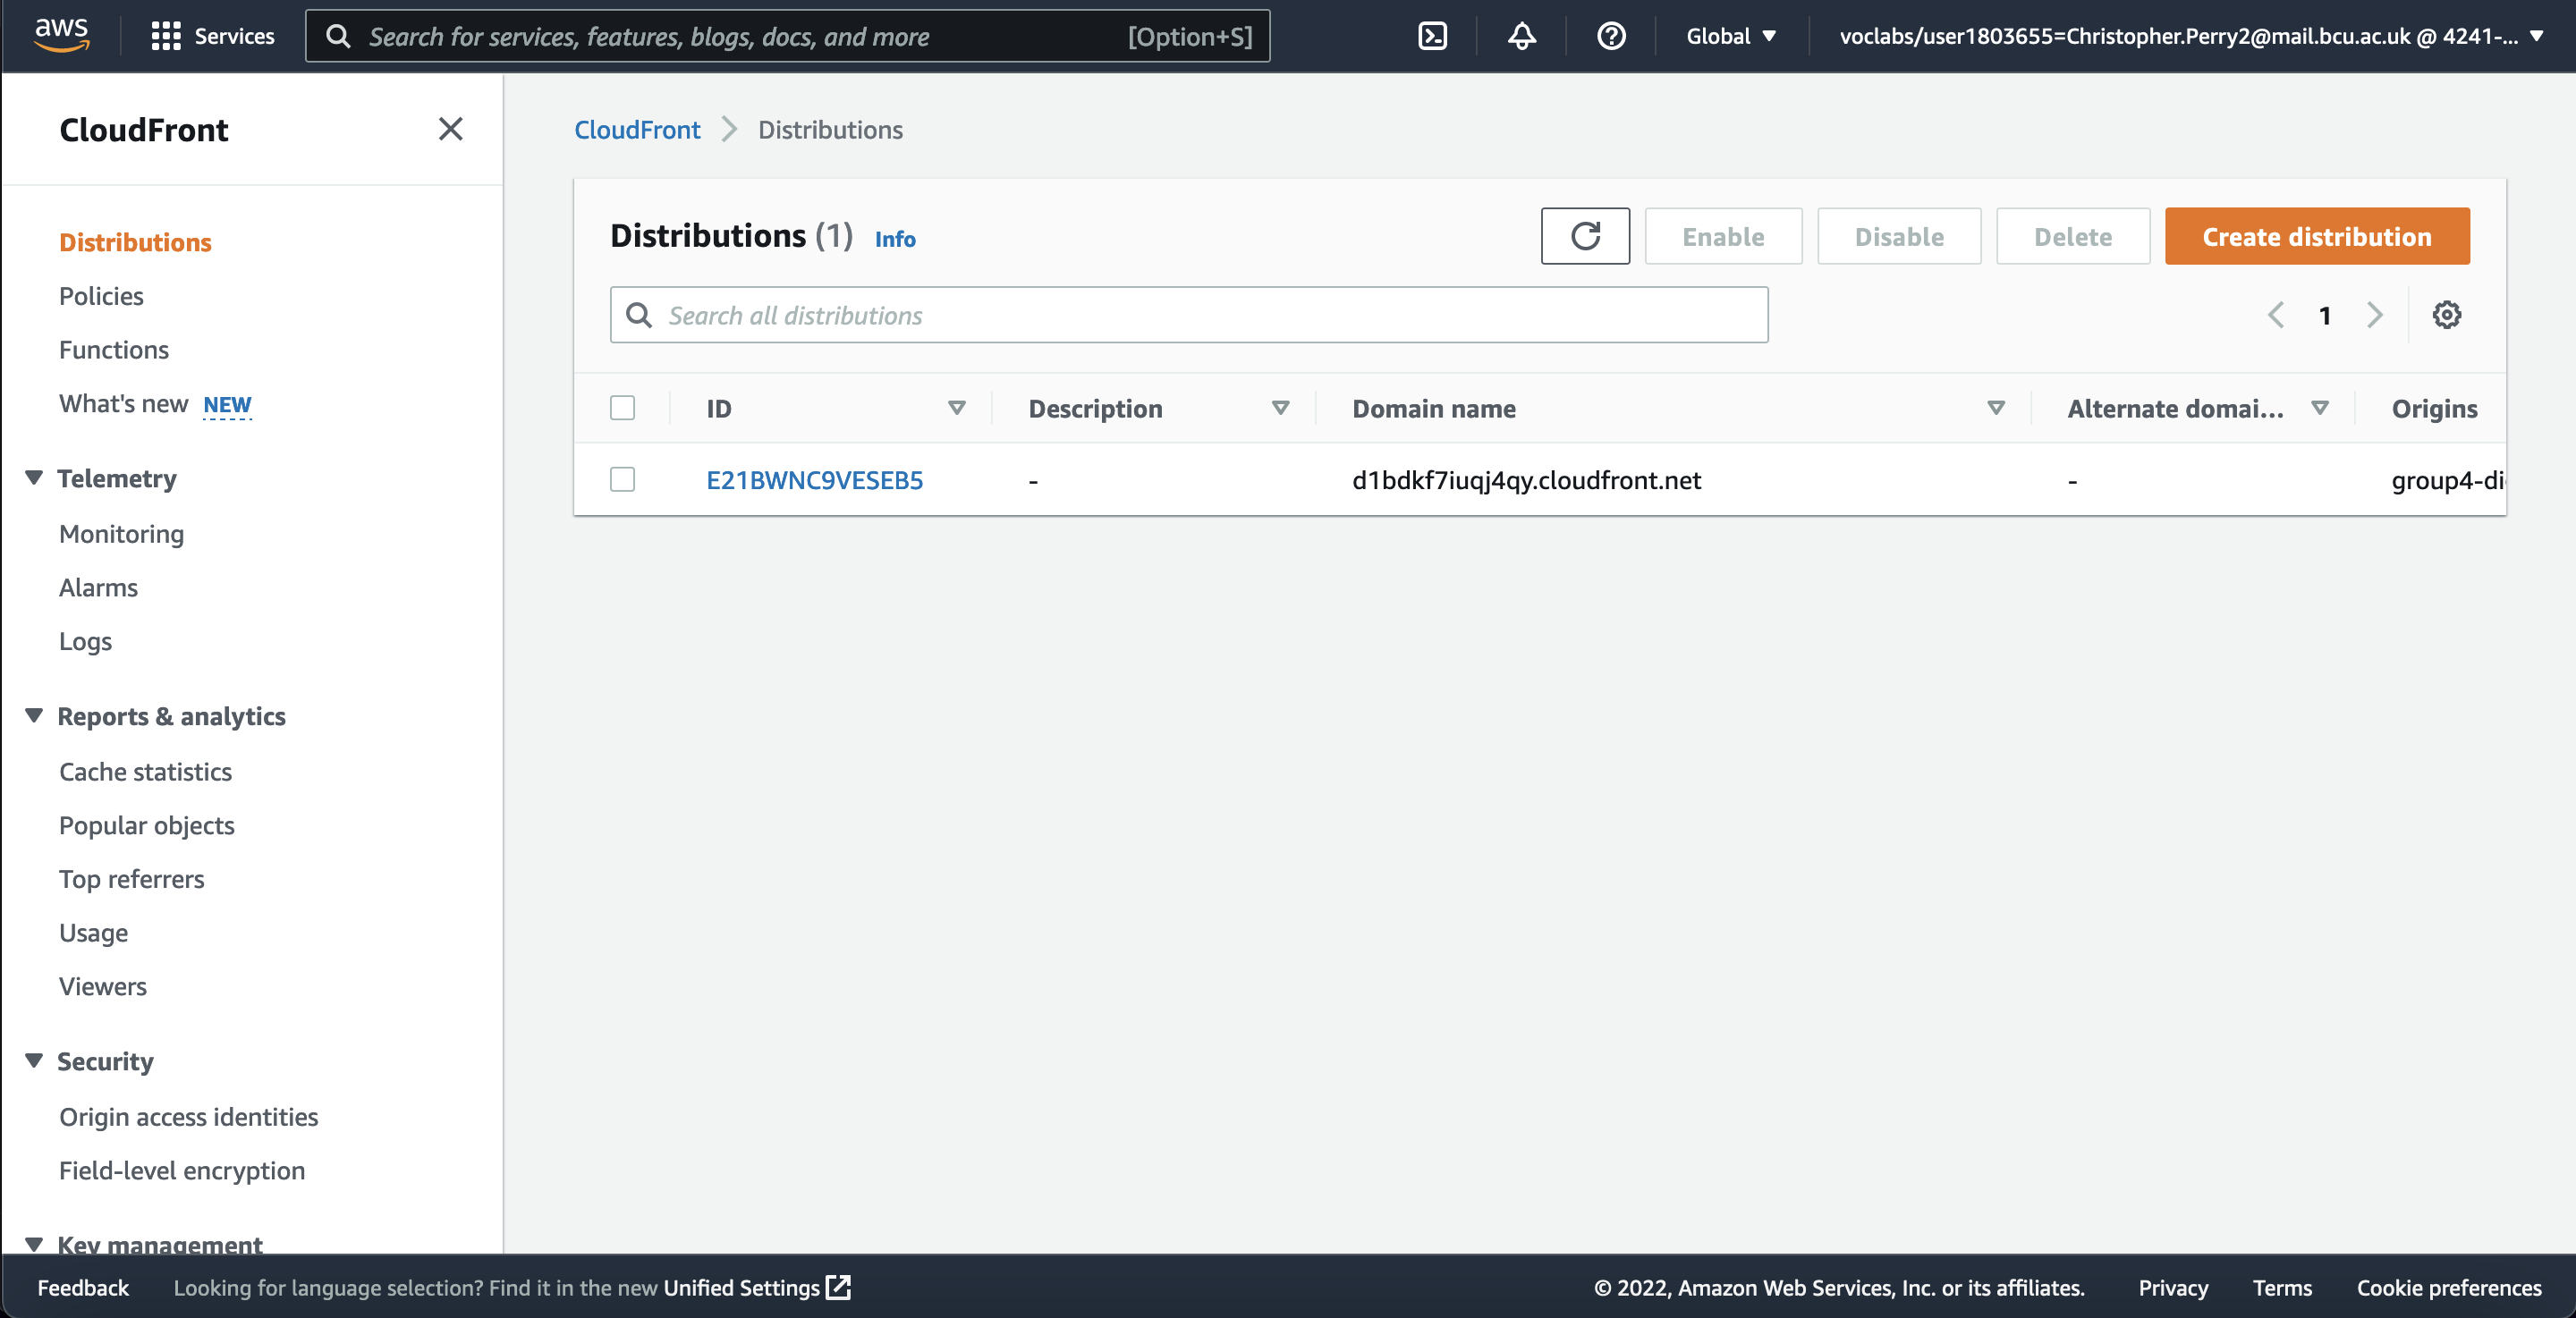
\includegraphics[width=\textwidth]{resources/cloudfront/cloudfront-created}
    \caption{Created CloudFront Distribution.}
    \label{fig:cloudfront-created}
\end{figure}

Finally, the images contained within the webserver were changed from their local location to their relevant CloudFront
locations.

\begin{figure}[!htbp]
    \centering
    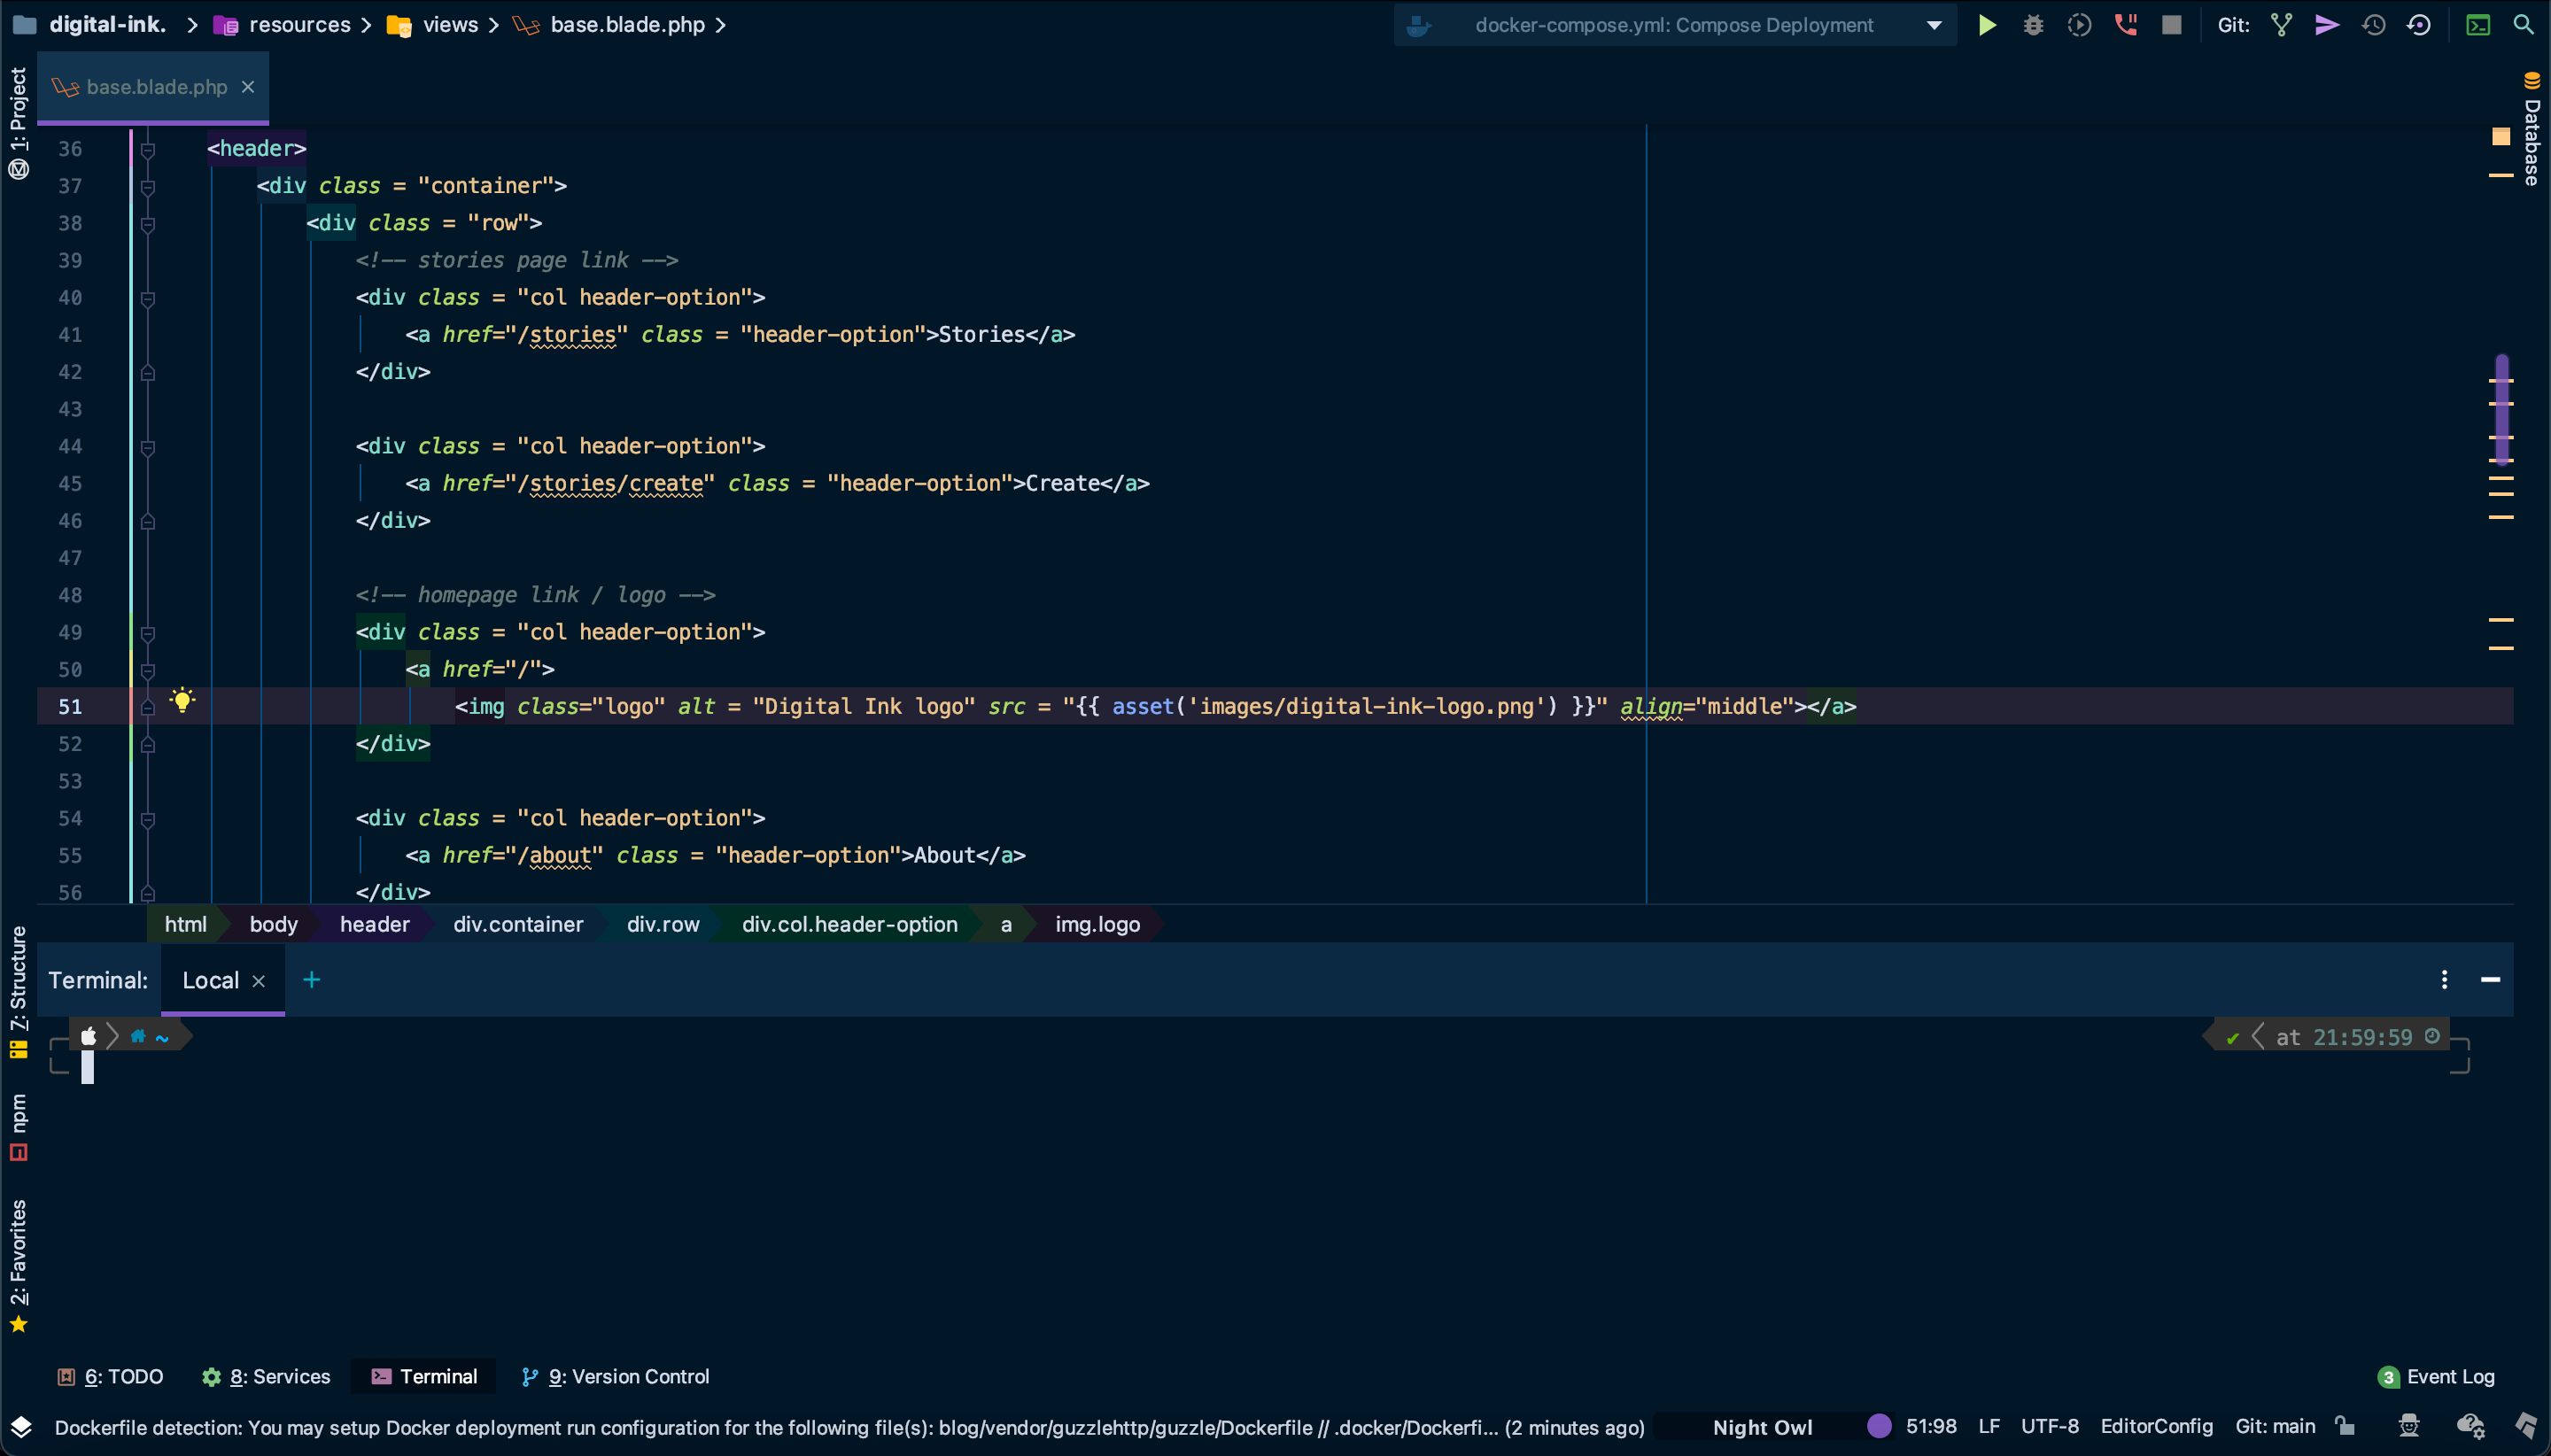
\includegraphics[width=\textwidth]{resources/cloudfront/cloudfront-before}
    \caption{Image location before CloudFront.}
    \label{fig:cloudfront-before}
\end{figure}

\begin{figure}[!htbp]
    \centering
    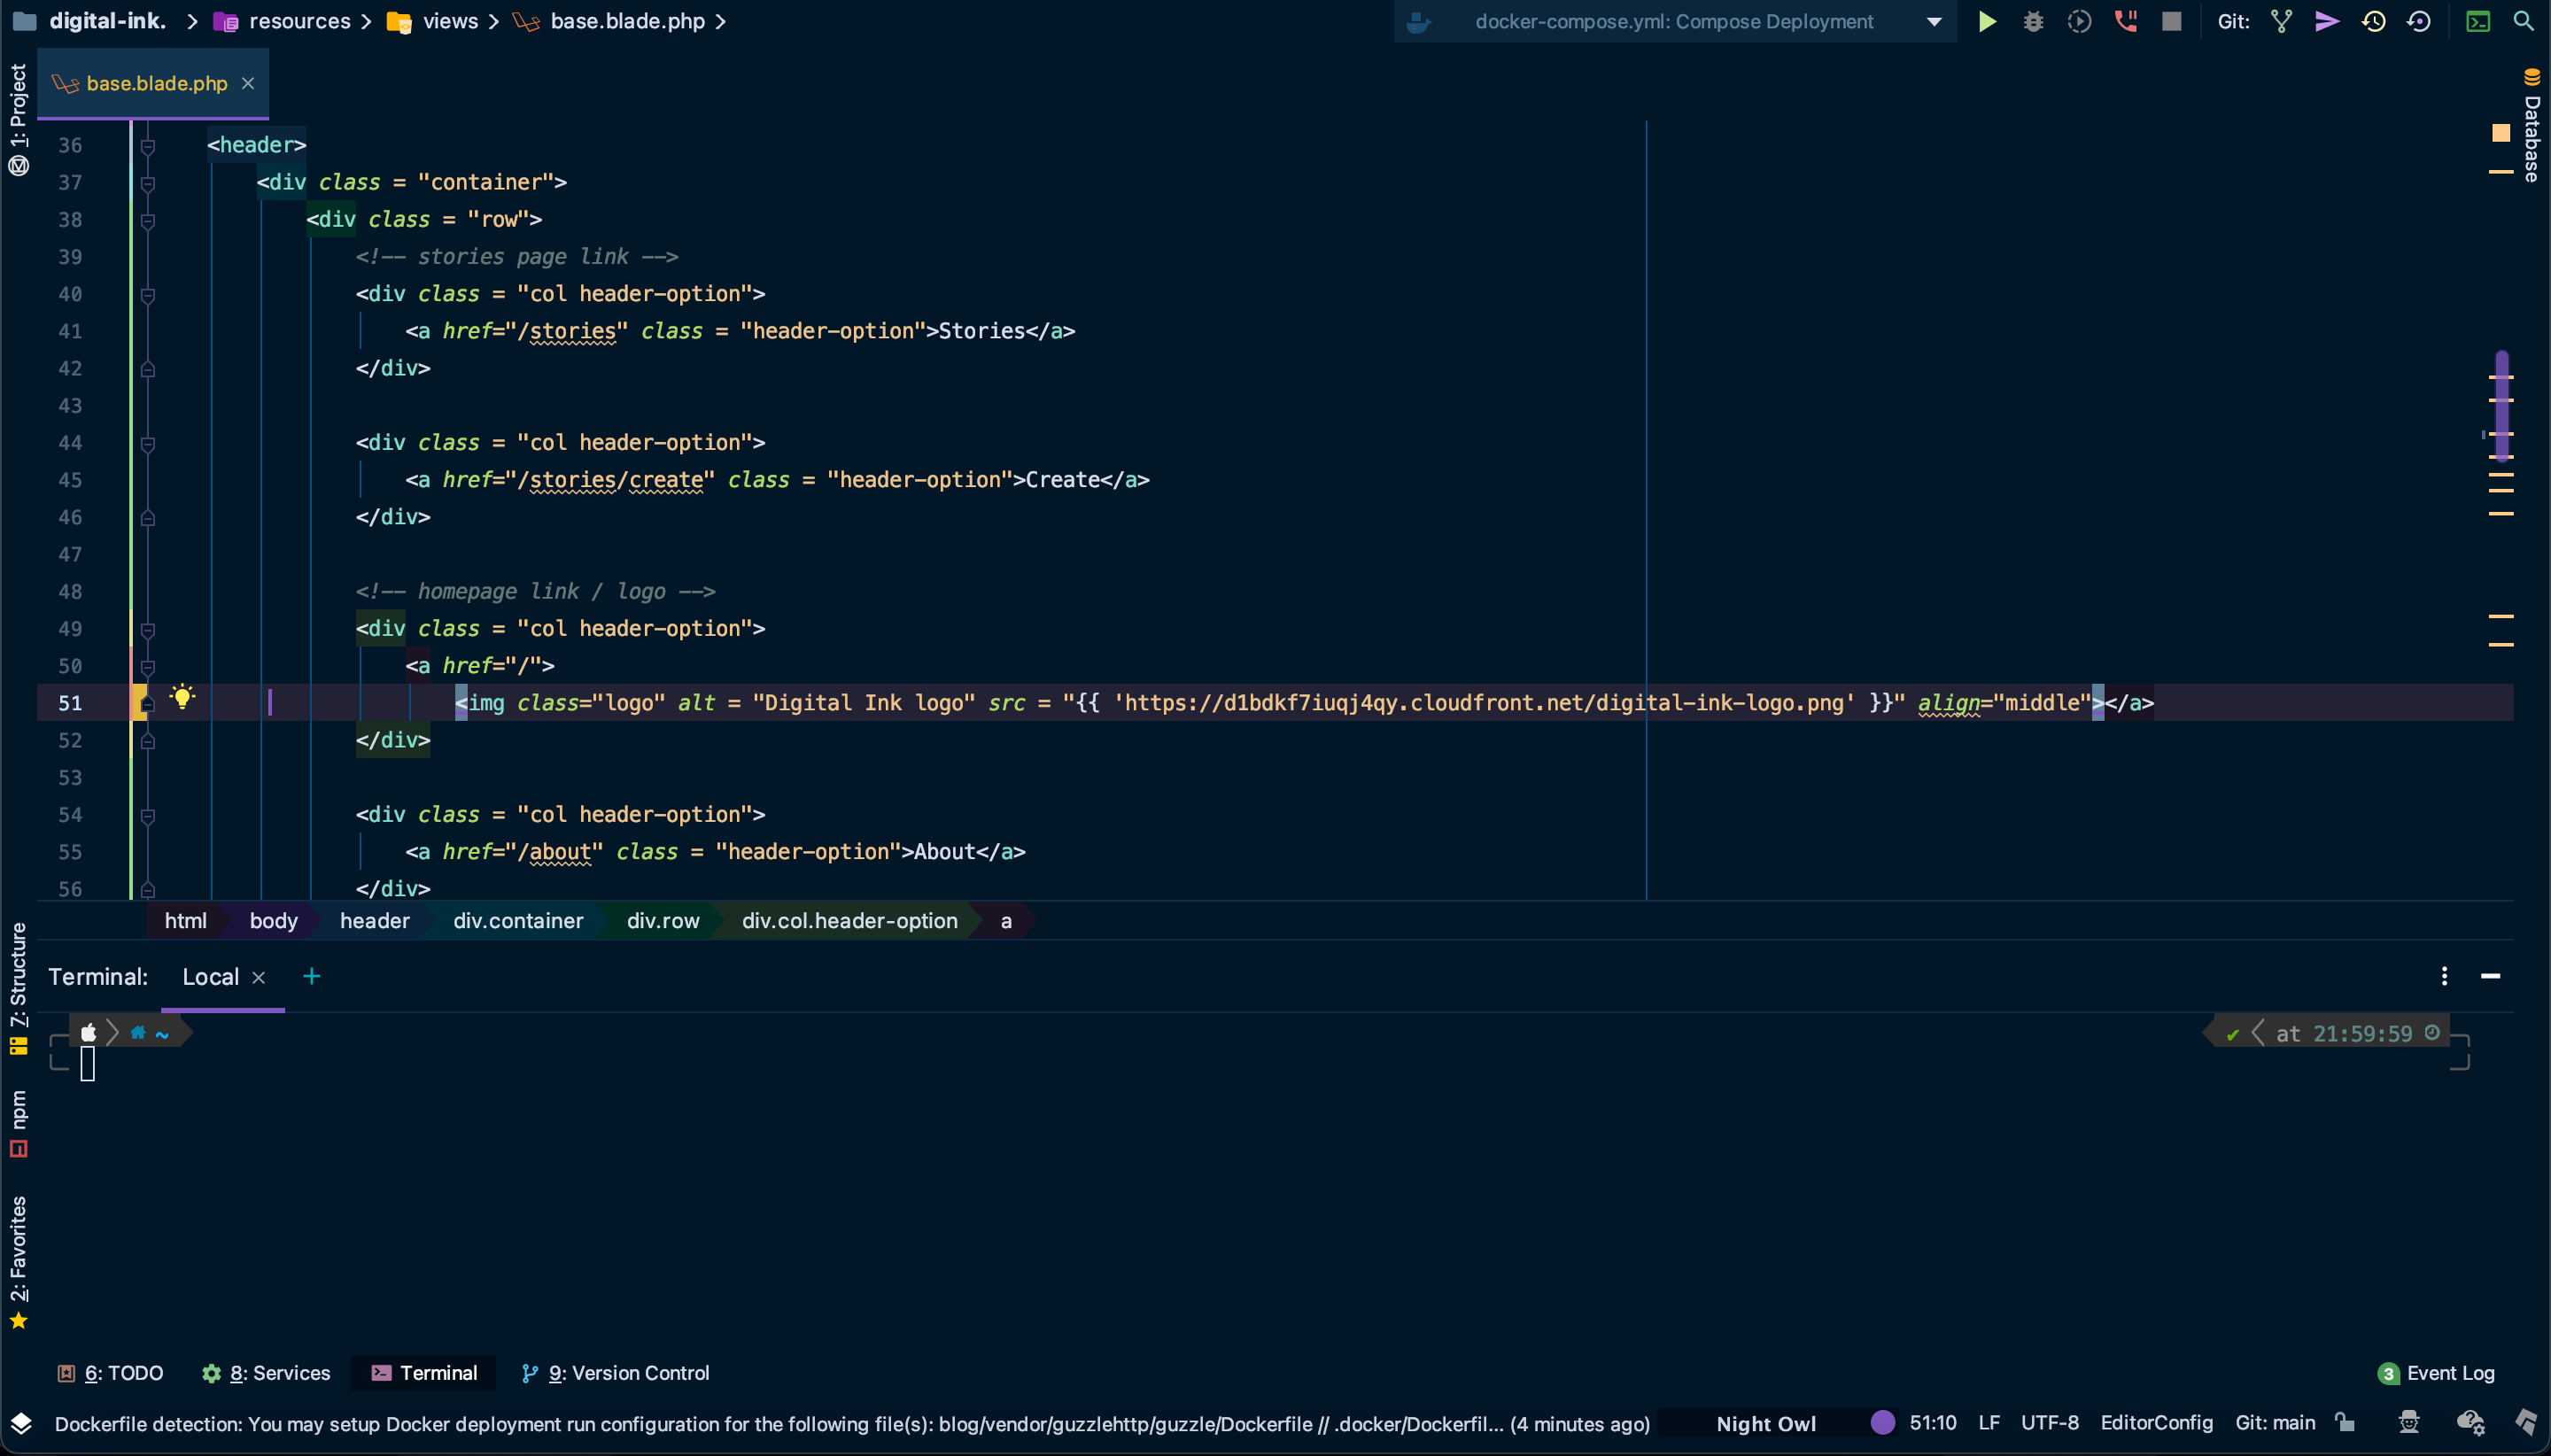
\includegraphics[width=\textwidth]{resources/cloudfront/cloudfront-after}
    \caption{Image location after CloudFront.}
    \label{fig:cloudfront-after}
\end{figure}





